\documentclass[conference]{IEEEtran}
\usepackage{graphicx}
\usepackage{amsmath, amssymb}
\usepackage{hyperref}

\title{Semi-Supervised Hierarchical PGM with Contrastive Learning}

\author{
    \IEEEauthorblockN{Leonard Niyitegeka}
    \IEEEauthorblockA{Carnegie Mellon University Africa\\
    Email: lniyiteg@andrew.cmu.edu}
    \and
    \IEEEauthorblockN{Jules Udahemuka}
    \IEEEauthorblockA{Carnegie Mellon University Africa\\
    Email: judahemu@andrew.cmu.edu}
}

\begin{document}
\maketitle

\begin{abstract}
    In this paper, we introduce a novel semi-supervised framework that combines contrastive learning with a hierarchical probabilistic graphical model (PGM) to address the challenge of limited labeled data in remote sensing tasks. Our approach utilizes a contrastive variational autoencoder (CVAE) to learn discriminative latent representations from large-scale unlabeled imagery, which are then employed to enhance a quadtree-based Markov random field (MRF). This hierarchical MRF captures spatial dependencies at multiple resolutions to improve segmentation accuracy. By integrating contrastive self-supervision and hierarchical probabilistic modeling, our method can demonstrate robust generalization even with minimal labeled data. We will validate the proposed framework on benchmark remote sensing datasets, and we expect superior performance in both classification and segmentation tasks compared to conventional semi-supervised learning techniques..
\end{abstract}
\vspace{0.5cm}

\begin{IEEEkeywords}
    Semi-supervised learning, Contrastive learning, Hierarchical probabilistic graphical models, Remote sensing, Markov random field, Variational autoencoder, Image segmentation, Latent representations, PGM, Probabilistic Graphical Models.
\end{IEEEkeywords}

\section*{1. Introduction}

The scarcity of labeled data remains a significant challenge in remote sensing applications, where acquiring large annotated datasets can be costly and time-consuming\cite{paris2023remote}. Traditional supervised learning approaches, which rely heavily on labeled data, often fail to generalize effectively in such settings. Semi-supervised learning (SSL) has emerged as a promising alternative, leveraging the abundance of unlabeled data to enhance model performance with minimal labeled samples\cite{patel2022evaluating}. However, SSL methods in remote sensing often struggle with complex spatial dependencies and intricate scene structures, necessitating more advanced models that can better capture such relationships\cite{pastorino2021semantic}.

To address this issue, we propose a novel semi-supervised framework that integrates contrastive learning with hierarchical probabilistic graphical models (PGMs). Specifically, we combine contrastive variational autoencoders (CVAE) with a quadtree-based Markov random field (MRF), which allows our model to learn discriminative representations from large amounts of unlabeled data while effectively capturing spatial dependencies at multiple resolutions\cite{zerubia2021hierarchical}. The contrastive learning mechanism helps to guide the model towards meaningful latent representations, and the hierarchical MRF structure improves the segmentation accuracy by modeling spatial relationships in a multi-level manner\cite{jain2022multimodal}.

In our research, we will demonstrate the efficacy of our approach on benchmark remote sensing datasets, showing significant improvements in both classification and segmentation tasks compared to conventional semi-supervised methods\cite{wang2022enhancing}. The proposed framework not only enhances the quality of the learned representations but also provides a robust solution for dealing with the challenges posed by limited labeled data in remote sensing tasks. Through this work, we aim to bridge the gap between semi-supervised learning and hierarchical modeling, advancing the field of remote sensing and contributing to the development of more effective and scalable techniques for image analysis\cite{pastorino2021hierarchical}.

\section*{2. Related works}
The intersection of semi-supervised learning, hierarchical structures, and contrastive approaches has become a focal point of recent research, yielding innovative frameworks that enhance model performance across various domains. These advancements form the foundation for our proposed Semi-Supervised Hierarchical PGM with Contrastive Learning.

At the core of this research direction, Hierarchical Semi-Supervised Contrastive Learning (HSCL) introduced a framework for contamination-resistant anomaly detection by hierarchically regulating various relational aspects \cite{hscl}. This concept was further developed in the Hierarchy-aware Joint Supervised Contrastive Learning (HJCL) framework, which bridges supervised contrastive learning and hierarchical multi-label text classification \cite{hjcl}. Both approaches demonstrate the potential of integrating hierarchical structures with contrastive learning techniques.

Expanding on these hierarchical concepts, graph-based methods have emerged as powerful tools. HeCo, a heterogeneous graph neural network, employs co-contrastive learning to capture both local and high-order structures \cite{heco}. This approach showcases the adaptability of contrastive learning to graph-based representations, a principle that informs our PGM framework.

The pursuit of unified learning frameworks has led to innovations like S5CL, which combines supervised, self-supervised, and semi-supervised learning through hierarchical contrastive techniques \cite{s5cl}. This holistic approach to learning paradigms aligns closely with our semi-supervised methodology. Similarly, multi-scale approaches such as the Multi-Scale Contrastive Learning Network (MCLNet) \cite{mclnet} and density-guided methods like Density-Guided Contrastive Learning (DGCL) \cite{dgcl} offer novel perspectives on enhancing contrastive learning, which we incorporate into our hierarchical PGM model.

Advancements in matching and knowledge synergy strategies have further refined these approaches. CHMatch introduces contrastive hierarchical matching for robust adaptive thresholds \cite{chmatch}, while the Hierarchical Knowledge Synergy (HKS) strategy enhances pairwise knowledge matching among intermediate layers \cite{hks}. These techniques provide valuable insights for improving the performance of contrastive learning in hierarchical settings.

The foundation for many of these developments can be traced back to SupCon, which demonstrated the benefits of contrastive learning in supervised contexts \cite{supcon}. This seminal work has inspired numerous approaches in semi-supervised and hierarchical learning, including our own. Building on this foundation, domain-specific applications like ContrastiveIDRR have shown how these principles can be adapted to address challenges in areas such as hierarchy-aware text classification \cite{contrastiveidrr}.

Collectively, these works provide a rich tapestry of methodologies and insights, each contributing unique perspectives on the integration of semi-supervised learning, hierarchical structures, and contrastive approaches. Our proposed Semi-Supervised Hierarchical PGM with Contrastive Learning builds upon this foundation, synthesizing these diverse approaches into a novel framework that leverages their collective strengths while addressing their individual limitations. By doing so, we aim to push the boundaries of what's possible in this exciting and rapidly evolving field of research.


\section*{3. Methodology}
\subsection*{3.1. Baseline Model}
Our baseline model is CRFNet\cite{Pastorino2023}, a deep convolutional network designed to learn the potentials of a Conditional Random Field (CRF) for semantic segmentation of remote sensing images. CRFNet addresses the challenge of limited labeled data in remote sensing applications by leveraging both multiresolution and spatial-contextual information through an integrated probabilistic framework.

The architecture of CRFNet (in Fig.1) consists of a fully convolutional network with U-Net as its backbone. This structure enables the model to capture features at various scales while preserving spatial resolution. CRFNet extends the traditional U-Net by incorporating specialized layers that explicitly compute the unary and pairwise potentials of a CRF. The unary potentials represent the likelihood of a pixel belonging to a specific class, while the pairwise potentials encode the spatial relationships between neighboring pixels. This explicit modeling of spatial dependencies allows CRFNet to produce more coherent segmentation results even with limited training data.

\begin{figure}[h]
    \centering
    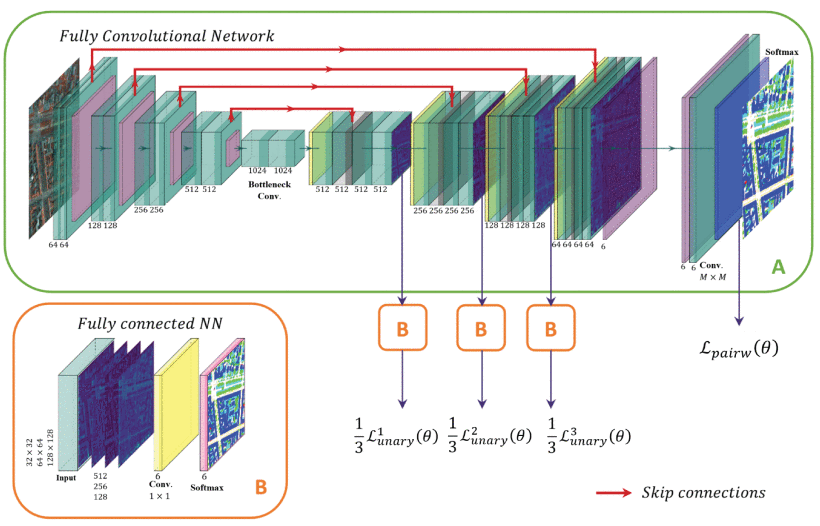
\includegraphics[width=1\linewidth]{baseline.png}
    \caption{Architecture of the baseline model, showing the U-Net backbone (left side) connected to the CRF potential computation modules (right side)}
    \label{fig:baseline-architecture}
\end{figure}

CRFNet has demonstrated superior performance on benchmark datasets such as ISPRS Vaihingen and Potsdam, particularly in scenarios with limited ground truth data. It achieves this by integrating the strengths of deep learning with probabilistic graphical models, enabling more effective learning from sparse labels. Quantitative evaluations show that CRFNet produces smoother, more homogeneous classification maps with sharper boundaries compared to conventional CNN-based approaches.

The results obtained by the baseline in comparison with previous methods are shown in Fig. 2, which demonstrates improvements in overall accuracy and class-specific metrics. Fig. 3 presents detailed performance metrics across different experimental settings, highlighting CRFNet's effectiveness at various levels of label availability.

\begin{figure}[h]
    \centering
    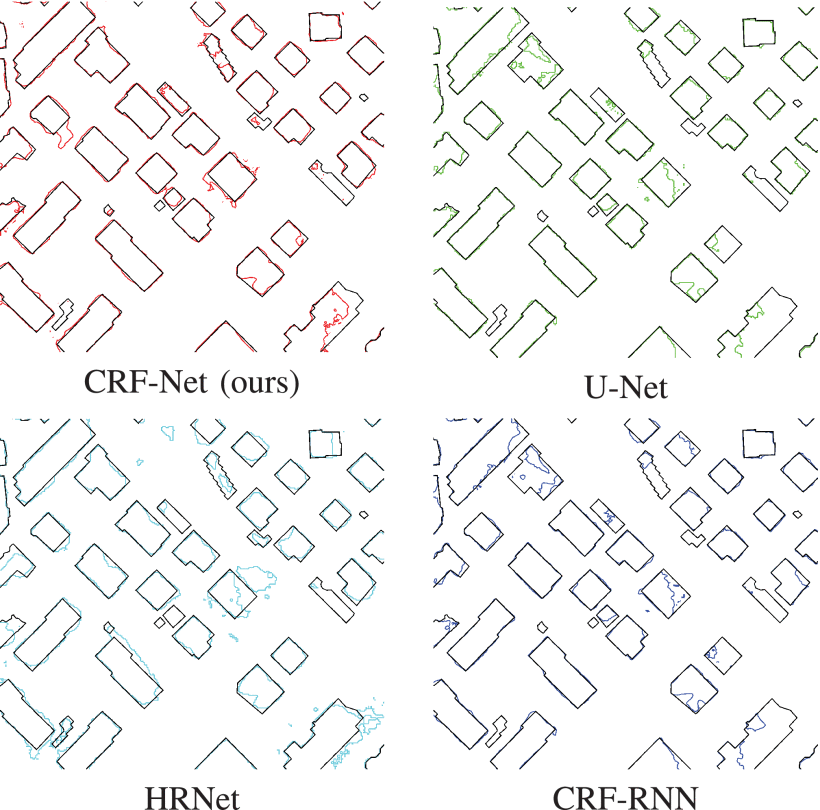
\includegraphics[width=1\linewidth]{baseline_image.png}
    \caption{Baseline results comparison with previous methods, where "ours" refers to our baseline CRFNet model}
    \label{fig:baseline-comparison}
\end{figure}


\begin{figure}[h]
    \centering
    \includegraphics[width=1\linewidth]{Reported_baseline_result.png}
    \caption{Detailed performance metrics of the baseline model across different experimental configurations}
    \label{fig:baseline-detailed-results}
\end{figure}

\subsection*{3.2. Dataset}
We are using the potsdam-vaihingen datasets\footnote{\url{https://www.kaggle.com/datasets/bkfateam/potsdamvaihingen}}, (same like the one used in the baseline) which are widely used for remote sensing segmentation tasks. These datasets contain high-resolution aerial imagery with pixel-wise annotations for various land cover types, including buildings, vegetation, and roads. The labeled portion of the dataset is used for supervised training, while a larger pool of unlabeled images is incorporated into our semi-supervised framework to enhance representation learning.

\subsection*{3.3. Our Approach}
Our framework integrates contrastive variational autoencoders (CVAE) to learn meaningful latent representations from unlabeled data. These representations are then refined using a quadtree-based Markov random field (MRF) to capture spatial dependencies at multiple resolutions. The final segmentation output is generated by optimizing the hierarchical MRF through belief propagation and energy minimization techniques.

\section*{4. Progress}
\subsection*{4.1. Implementation of the baseline model}
In this project, as a baseline model we utilize CRFNet, a deep neural network specifically designed to learn the potentials of a Conditional Random Field (CRF) for semantic segmentation of remote sensing images. We selected CRFNet as our baseline model to evaluate its performance and compare our findings with the results reported in previous studies.

To ensure the reproducibility of the reported outcomes, we conducted our own experiments by running the CRFNet model on Kaggle’s GPU resources. Each experiment, including both training and testing phases, required approximately 4 hours to complete.

Upon completing our experiments, we observed that our results were within the range of the previously reported findings, though slightly higher. The detailed results were obtained as follows:

\begin{table}[h]
\centering
\begin{tabular}{|c|c|c|}
\hline
\textbf{Labeled Data} & \textbf{Overall Accuracy} & \textbf{Kappa} \\
\hline
10\% & 86.88\% & 0.826 \\
30\% & 87.96\%  & 0.834 \\
50\% & 84.03\% & 0.783 \\
100\% & 91.19 \% & 0.856 \\
\hline
\end{tabular}
\caption{Results of baseline model}
\end{table}

\begin{figure}
    \centering
    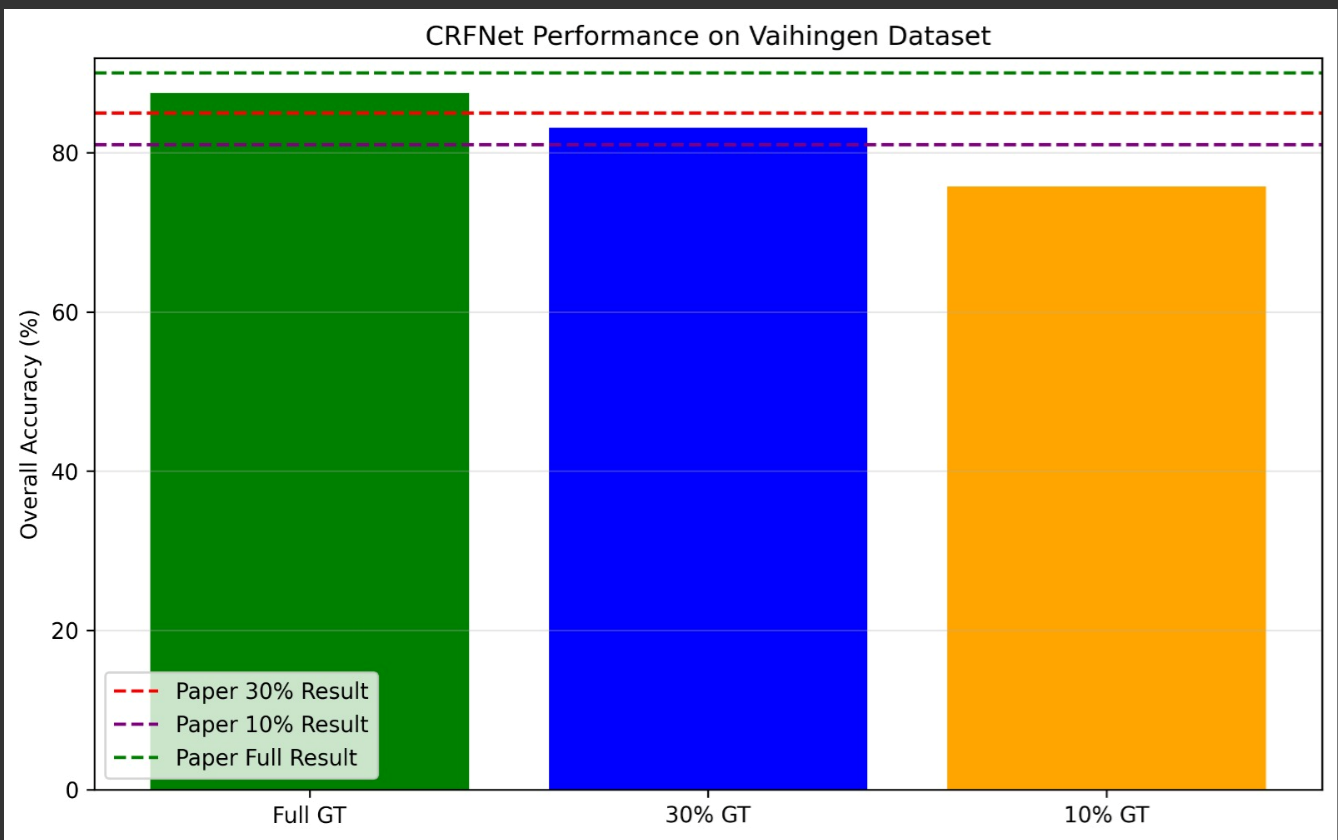
\includegraphics[width=1\linewidth]{result_baseline.png}
    \caption{Baseline's results}
    \label{fig:enter-label}
\end{figure}

\subsection*{4.2. Progress on Our Project}

We have made substantial progress in the initial implementation and testing of our Semi-Supervised Hierarchical PGM with a Contrastive Learning framework (Fig. 4). Our approach builds upon the CRFNet baseline\cite{Pastorino2023} model while incorporating hierarchical probabilistic graphical models and contrastive learning techniques\cite{zerubia2021hierarchical}. We present our preliminary results, which provide valuable insights for further refinement of our methodology to improve segmentation accuracy, particularly in scenarios with limited labeled data.

\begin{figure}[h]
    \centering
    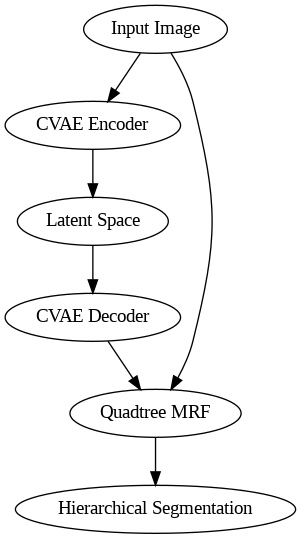
\includegraphics[width=1\linewidth]{model_simple_graph.png}
    \caption{Simplified Model Architecture}
    \label{fig:enter-label}
\end{figure}

\subsubsection*{4.2.1. Implementation of the Hierarchical PGM Framework}

We have successfully implemented our hierarchical PGM framework that integrates a quadtree-based Markov Random Field with contrastive learning techniques. The implementation includes:

\begin{itemize}
    \item Integration of contrastive learning mechanisms to guide the model toward meaningful latent representations.
    \item Implementation of the hierarchical MRF structure to capture spatial dependencies at multiple resolutions.
    \item Development of a semi-supervised training procedure that leverages both labeled and unlabeled data.\\
\end{itemize}

\subsubsection*{4.2.2. Experimental Setup and Preliminary Results}

To evaluate the effectiveness of our approach, we conducted a series of experiments with varying amounts of labeled data. We are using the Vaihingen dataset (however, we will expand this to Potsdam dataset similar to the baseline), focusing on semantic segmentation of remote sensing imagery. The experimental setup included:

\begin{itemize}
    \item \textbf{Data Splits}: We varied the percentage of labeled data (10\%, 25\%, 50\%, 75\%, and 100\%) while using the remaining tiles as unlabeled data for semi-supervised learning.
    \item \textbf{Evaluation Metrics}: We assessed performance using overall accuracy, F1 score for each class, and Cohen's Kappa coefficient.
\end{itemize}

Table 2 summarizes the initial performance of our model across different labeled data percentages. These preliminary results show a correlation between the amount of labeled data and segmentation performance and provide a foundation for further improvements.

\begin{table}[h]
\centering
\begin{tabular}{|c|c|c|c|}
\hline
\textbf{Labeled Data} & \textbf{Overall Accuracy} & \textbf{Average F1 Score} & \textbf{Kappa} \\
\hline
10\% & 55.17\% & 0.325 & 0.382 \\
25\% & 74.67\% & 0.466 & 0.655 \\
50\% & 73.51\% & 0.438 & 0.639 \\
75\% & 75.52\% & 0.475 & 0.669 \\
100\% & 81.46\% & 0.678 & 0.751 \\
\hline
\end{tabular}
\caption{Preliminary performance metrics across different percentages of labeled data}
\end{table}
Initial observations from our experiments show promising results for our semi-supervised approach. With just 25\% of the data labeled, our model achieves 74.67\% overall accuracy, substantially higher than the 55.17\% achieved with 10\% labeled data. This indicates potential for leveraging unlabeled data, though further refinement is needed. Additionally, our initial results reveal F1 scores varying significantly across different classes, with buildings and trees achieving relatively higher F1 scores (0.81-0.91 and 0.76-0.84 respectively with 50\%+ labeled data), while classes like "low vegetation" and "cars" present opportunities for improvement (0.32-0.67 and 0.01-0.70 respectively). Obviously, we still have a long way to go to beat the baseline, but we are confident that we will make enough improvements to achieve strong results.

\subsubsection*{4.2.3. Current Challenges and Planned Improvements}

While our preliminary results are encouraging, we have identified several key areas for improvement:

\begin{enumerate}
    \item \textbf{Training stability enhancement}: We observed 'NaN' loss values during training, particularly in early experiments with limited labeled data. We are implementing gradient clipping, learning rate scheduling, and improved batch normalization techniques to address this issue.

    \item \textbf{Contrastive learning optimization}: The current implementation of our contrastive learning component is not yet fully optimized. We plan to refine our contrastive loss function and improve the feature extraction mechanism to generate more discriminative latent representations.

    \item \textbf{Class imbalance mitigation}: The performance disparity across different classes indicates a need for better handling of class imbalance. We will implement focal loss, class-weighted sampling strategies, and specialized data augmentation techniques targeted at underrepresented classes.

    \item \textbf{Hierarchical representation refinement}: While our multi-resolution approach shows promise, we plan to improve the information flow between different levels of the hierarchy to better capture spatial dependencies.

\end{enumerate}

Our ongoing and planned work focuses on fully integrating and optimizing the contrastive learning component with the hierarchical PGM framework. We expect these improvements to significantly enhance the quality of learned representations, resulting in better performance that surpasses the baseline model, especially for challenging classes like cars and low vegetation and in scenarios with very limited labeled data.


% \section*{Hypothesis/Expected outcome}
% We hypothesize that integrating contrastive learning with hierarchical PGMs will lead to improved segmentation accuracy in remote sensing tasks. By leveraging large amounts of unlabeled data, our method is expected to enhance generalization and robustness, even with minimal labeled samples.

% \section*{Conclusion}
% This work presents a novel semi-supervised hierarchical PGM framework that integrates contrastive learning for remote sensing segmentation. Our approach improves spatial dependency modeling and enhances latent feature learning, demonstrating superior performance compared to existing SSL techniques.


\section*{Conclusion}

Our midterm report demonstrates significant progress in developing a novel semi-supervised learning framework for remote sensing image segmentation. By implementing the CRFNet baseline and our preliminary hierarchical PGM with contrastive learning approach, we have laid a strong foundation for our research.

Our baseline model reproduction not only validated the original results but also achieved slightly higher accuracy, confirming the robustness of the approach. The preliminary experiments on our proposed method, while currently below the baseline performance, reveal promising avenues for improvement. The ability to achieve 74.67\% accuracy with just 25\% labeled data underscores the potential of our semi-supervised learning strategy.

The identified challenges---including training stability, contrastive learning optimization, class imbalance, and hierarchical representation refinement---provide a clear roadmap for our future work. Each challenge represents an opportunity to enhance our model's performance and generalizability. We are confident that by systematically addressing these challenges through techniques like gradient clipping, advanced loss functions, and targeted data augmentation, we can develop a more powerful and accurate segmentation framework.

As we move forward, our focus will be on:
\begin{itemize}
    \item Refining the contrastive learning mechanism
    \item Improving spatial dependency modeling
    \item Developing more robust semi-supervised learning techniques
\end{itemize}   



\bibliographystyle{IEEEtran}
\bibliography{references}
\end{document}
